\section{Resultados, Lições Aprendidas e Limitações}
\label{sec:resultados}

Os experimentos usaram a v2.2.1. A v2.2.2 só acrescenta ao texto a recomendação de 4 jogadores, e as suas
partidas são as mesmas da v2.2.1 (um teste automático confere isso evento a evento). Por isso os resultados
valem para a versão atual.

\subsection{QP1: a v2 reduz o desequilíbrio da v1?}

\textbf{A v1 simulada reproduz o mecanismo do artigo.} Na v1 simulada, quem lidera depois que todos fizeram o
primeiro teste vence entre 49\% e 78\% das partidas, conforme a população de bots. Pelo critério fixado antes do
experimento (vencedor com pelo menos 1,5 vez a média dos demais), mais de 95\% das partidas da v1 simulada são
desequilibradas, contra 4 de 6 no artigo. Com o fator 2,0, as populações mais parecidas com estudantes ficam
dentro do intervalo de confiança das 6 partidas do artigo (de 0,30 a 0,90).
% fonte: resultados/fase3_exp1_validacao_v1/20261110-205949-ad1624f/relatorio.md
O simulador também explica por que atacar o líder não freava a bola de neve na v1. Lá, a defesa bem-sucedida
entregava a carta de ataque ao defensor; como o líder tem um sistema grande e quase sempre tem a categoria
atacada, quem o atacava o alimentava. Para os bots, escolher o alvo ao acaso foi a melhor resposta.

\textbf{A v2 quase elimina a vantagem do líder.} Com os mesmos bots, as mesmas mesas e as mesmas sementes nas duas
versões, a vantagem do líder (REQ-02) cai de 0,392 para 0,087 com 4 jogadores e de 0,419 para 0,091 com 5
(Figura~\ref{fig:lider}). As diferenças são de 0,305 (intervalo de 0,290 a 0,319) e de 0,328 (de 0,316 a 0,342),
bem acima da margem de 0,05 exigida. Na v2, atacar o líder passa a ser a melhor política entre os Caçadores, e
atacar o mais fraco, a pior: o contrário da v1.
% fonte: resultados/fase3_exp2_v1_contra_v2/20261110-212034-f447f4b/relatorio.md

\begin{figure}[ht]
  \centering
  % Vantagem do líder (REQ-02): v1 contra v2.2.1, mesmas mesas mistas e mesmas sementes.
% fonte: resultados/fase3_exp2_v1_contra_v2/20261110-212034-f447f4b/relatorio.md
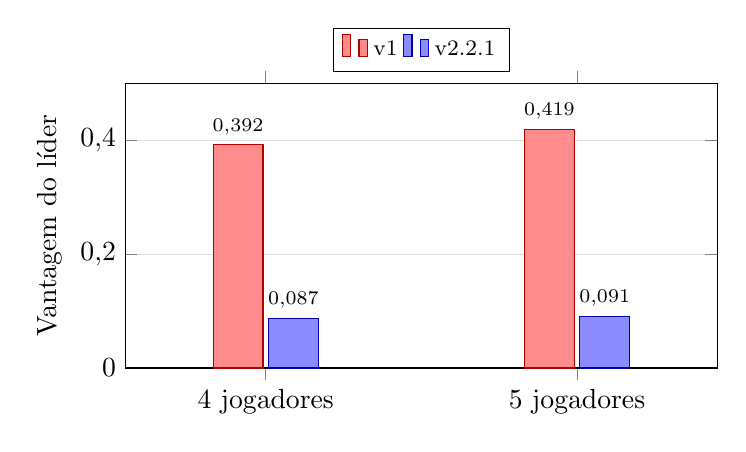
\begin{tikzpicture}
  \begin{axis}[
      ybar,
      bar width=18pt,
      width=0.75\linewidth,
      height=5.2cm,
      ymin=0, ymax=0.5,
      ylabel={Vantagem do líder},
      symbolic x coords={4 jogadores,5 jogadores},
      xtick=data,
      enlarge x limits=0.45,
      legend style={at={(0.5,1.04)}, anchor=south, legend columns=-1, font=\footnotesize},
      nodes near coords,
      every node near coord/.append style={font=\scriptsize, /pgf/number format/fixed,
        /pgf/number format/precision=3, /pgf/number format/use comma},
      yticklabel style={/pgf/number format/fixed, /pgf/number format/use comma},
      ymajorgrids=true,
      grid style={gray!25},
    ]
    \addplot[fill=red!45, draw=red!70!black] coordinates {(4 jogadores,0.392) (5 jogadores,0.419)};
    \addplot[fill=blue!45, draw=blue!70!black] coordinates {(4 jogadores,0.087) (5 jogadores,0.091)};
    \legend{v1, v2.2.1}
  \end{axis}
\end{tikzpicture}

  \caption{Vantagem do líder isolado após o ciclo 1 (chance de vencer menos $1/N$), na v1 e na v2.2.1}
  \label{fig:lider}
\end{figure}

\textbf{O melhor estilo é o Heurístico, que mistura construir e atacar.} A Tabela~\ref{tab:estilos} mostra a
taxa de vitória de um jogador de cada estilo (linha) numa mesa em que os outros três são de outro estilo
(coluna). O Heurístico é a melhor resposta, sozinho ou empatado, contra todas as mesas, menos a de Aleatórios. A
dinâmica do replicador termina em 100\% de Heurísticos, com 4 e com 5 jogadores. Nenhum Caçador puro é a melhor
resposta a mesa alguma, salvo a de Aleatórios: na v2.2.1, construir rende mais que caçar. Mesmo assim, os dois
estilos aparecem no jogo de quem joga bem. O Heurístico enche o sistema no 1º Planejamento em cerca de metade das
partidas e, nas outras, guarda cartas para testar (REQ-11). Habilidade importa: o Heurístico vence 0,938 das
partidas contra três Aleatórios, bem acima do piso de 0,375 (REQ-03).
% fonte: resultados/fase4_melhor_estilo/20261110-221516-ccd5649/relatorio.md

\begin{table}[ht]
  \centering
  \caption{Taxa de vitória do estilo da linha numa mesa com 3 jogadores do estilo da coluna (4 jogadores;
    referência 0,250; intervalos de cerca de $\pm 0{,}02$). Em negrito, as melhores respostas de cada coluna}
  \label{tab:estilos}
  \footnotesize
  \begin{tabular}{l c c c c c c}
    \toprule
    Estilo $\backslash$ Mesa & Aleatório & Construtor & Heurístico & Caç.\ líder & Caç.\ fraco & Caç.\ acaso \\
    \midrule
    Aleatório & 0,250 & 0,001 & 0,002 & 0,055 & 0,004 & 0,004 \\
    Construtor & \textbf{0,973} & \textbf{0,250} & \textbf{0,239} & \textbf{0,531} & 0,383 & \textbf{0,427} \\
    Heurístico & 0,938 & \textbf{0,264} & \textbf{0,250} & \textbf{0,549} & \textbf{0,434} & \textbf{0,451} \\
    Caçador (líder) & \textbf{0,965} & 0,168 & 0,113 & 0,250 & 0,387 & 0,294 \\
    Caçador (mais fraco) & 0,925 & 0,134 & 0,083 & 0,202 & 0,250 & 0,203 \\
    Caçador (ao acaso) & 0,943 & 0,146 & 0,087 & 0,234 & 0,325 & 0,250 \\
    \bottomrule
  \end{tabular}
\end{table}

\textbf{O blefe está equilibrado.} Num torneio entre 9 perfis puros de blefe (blefar nunca, metade das vezes ou
sempre; contestar nunca, sempre ou pelo limiar), nenhum perfil domina, e os perfis formam um ciclo. Blefar sempre
ganha de quem nunca contesta, contestar pelo limiar ganha de quem blefa, e não contestar ganha numa mesa de
honestos. O equilíbrio é uma mistura em que cerca de 1 em cada 6 jogadores blefa sempre. Nessa mistura, 39,5\% dos
blefes dão certo com 4 jogadores (intervalo de 38,6\% a 40,3\%) e 38,5\% com 5, dentro da faixa de 30\% a 50\% que
as regras pedem (REQ-05).
% fonte: resultados/fase4_exp5_blefe/20261110-231109-b02b6d4 e fase4_exp5b_blefe_equilibrio/20261111-004253-e17bbf2

\subsection{Requisitos, variantes e profundidade}

A Tabela~\ref{tab:resultados} resume os 13 requisitos, medidos com mesas de Heurísticos sorteadas do equilíbrio
do blefe, com conhecimento iniciante e experiente. Dez passam, dois passam em parte e um falha.

\begin{table}[ht]
  \centering
  \caption{Resultado dos requisitos na v2.2.1 (4 e 5 jogadores; iniciantes e experientes)}
  \label{tab:resultados}
  \footnotesize
  \begin{tabularx}{\linewidth}{>{\raggedright\arraybackslash}p{3.4cm} >{\raggedright\arraybackslash}p{1.6cm} >{\raggedright\arraybackslash}X}
    \toprule
    Requisito & Resultado & Valor medido \\
    \midrule
    REQ-01 Equidade de assento & em parte & Com bots aleatórios, todas as posições passam. Com Heurísticos, o 1º vence 0,276 e o último 0,224 (4 jogadores), na borda da zona \\
    REQ-02 Anti bola de neve & passa & 0,39 na v1 contra 0,09 na v2 \\
    REQ-03 Habilidade importa & passa & 0,938 (4 jog.) e 0,926 (5 jog.) \\
    REQ-04 Sem estratégia dominante & passa & Nenhum estilo nem perfil de blefe domina \\
    REQ-05 Blefes bem-sucedidos & passa & 0,395 e 0,385 \\
    REQ-06 Distribuição de ataques & passa & Razão de 1,35 a 1,43; fração contra o menor perto do limite com experientes \\
    REQ-07 Fichas não zeram cedo & passa & De 0,03 a 0,08 \\
    REQ-08 Duração & em parte & 44 min com 5 jogadores (passa); 38 min com 4 (abaixo de 40) \\
    REQ-09 Robustez & passa & 0 falhas em 971 mil partidas \\
    REQ-10 Tempo parado & \textbf{falha} & Percentil 90 de 5,8 min (4 jog.) e 9,0 min (5 jog.) \\
    REQ-11 Os dois estilos aparecem & passa & De 0,50 a 0,58 \\
    REQ-12 O 1º incidente não decide & passa & De 0,03 a 0,08 \\
    REQ-13 Incidentes pesam & passa & 0,29 (iniciantes) e 0,32 (experientes) \\
    \bottomrule
  \end{tabularx}
\end{table}

\textbf{Tempo e duração dependem de tempos ainda estimados.} Os tempos do modelo de duração são provisórios.
Com todos eles 25\% maiores, a partida de 4 jogadores passa a durar 48 minutos; com todos 25\% menores, o tempo
parado com 4 jogadores passa a 4,3 minutos. O resultado que não depende dos tempos é a relação entre os tamanhos de
mesa: a de 5 jogadores dura cerca de 15\% mais e fica cerca de 55\% mais tempo parada que a de 4. Por isso, a
v2.2.2 recomenda 4 jogadores (COR-03), mantendo o limite de 5.
% fonte: resultados/fase4_exp4_sensibilidade/20261111-082054-73762b5/relatorio.md

\textbf{O peso dos incidentes depende do conhecimento.} Medido só pelo dano, o peso dos incidentes era de 0,22
com iniciantes e de 0,17 com experientes, abaixo da zona. Quem sabe o conteúdo diagnostica melhor e se cobre
melhor, e por isso perde menos. Mas ganha mais no próprio incidente: pelos perfis do simulador, o experiente acerta o diagnóstico em 80\%
das vezes, e o iniciante em 40\%. Contando o incidente inteiro (dano e ganho do diagnóstico), o peso é de
0,29 com iniciantes e de 0,32 com experientes, e o requisito passa nos 40 cenários do Experimento 6. Essa
definição foi adotada pelo autor depois da primeira medição. A medida só pelo dano continua nos relatórios como
descrição.
% fonte: resultados/fase4_exp6_variantes/20261114-145900-0564baa/relatorio.md

\textbf{Nenhuma variante melhora tudo.} Das variantes propostas para o playtest:
\begin{itemize}
  \item comprar 2 cartas por Planejamento torna impossível encher o sistema no ciclo 1;
  \item cobrar uma ficha a mais pela explicação errada faz os iniciantes zerarem cedo;
  \item um Auditor externo, que não joga, piora o tempo parado;
  \item o vizinho designado e o limite de 2 testes recebidos encurtam a partida, mas concentram os ataques;
  \item a punição do blefe com 0 ou 2 fichas, o palpite da plateia e o módulo quase não mudam o que o simulador
    mede.
\end{itemize}
A regra atual foi a melhor das 10 configurações no conjunto. A ablação mostrou que cada mudança da 2.2, quando
desfeita, piora algum requisito ou não melhora nenhum. Com 6 jogadores (sem a COR-01), a mediana passa de 50
minutos, e o tempo parado chega a 12 minutos por ciclo. Com o bug duplicado permitido (regra da 2.1), os ataques
se concentram. Na sensibilidade, 5 fichas iniciais é o mínimo que passa no REQ-07: com 4 fichas, de 13\% a 23\% das
partidas têm alguém zerado antes do ciclo 3.
% fonte: fase4_exp6_variantes, fase4_exp3_ablacao/20261111-080955-f925943, fase4_exp4_sensibilidade, fase4_exp4b_combinacoes/20261111-134424-b263c34

\textbf{Testes sem limite dão o jogo mais profundo.} O Experimento 7 comparou a regra atual com 1 e 2 testes por
ciclo e com um custo de 1 ficha a partir do 2º teste do ciclo (Tabela~\ref{tab:profundidade}). Os testes sem
limite dão:
\begin{itemize}
  \item o maior número de decisões e de defesas por jogador;
  \item a menor vantagem do líder;
  \item a maior chance de recuperação de quem não lidera após o ciclo 1;
  \item o maior retorno para quem joga bem, medido pela vitória de um Heurístico normal contra Heurísticos mais
    descuidados (temperatura 4).
\end{itemize}
Com 1 teste por ciclo, a partida fica cerca de 10 minutos mais curta, mas é a regra mais rasa em todas as
medidas.
% fonte: resultados/fase4_exp7_profundidade/20261111-183119-3a2f2e0/relatorio.md

\begin{table}[ht]
  \centering
  \caption{Profundidade das regras de teste. Duração mediana em minutos com 4 e 5 jogadores; defesas e decisões
    por jogador; vantagem do líder (faixa entre iniciantes e experientes); ``jogar bem'': vitória do jogador
    cuidadoso dividida por $1/N$ contra jogadores descuidados, com 4 e 5 jogadores}
  \label{tab:profundidade}
  \footnotesize
  \setlength{\tabcolsep}{4pt}
  \begin{tabular}{l c c c c c}
    \toprule
    Regra & Duração & Defesas & Decisões & Vantagem do líder & Jogar bem \\
    \midrule
    \textbf{Sem limite (atual)} & 38 / 44 & \textbf{5,5} & \textbf{33} & \textbf{0,15--0,19} & \textbf{1,88 / 2,10} \\
    Custo a partir do 2º teste & 34 / 39 & 4,1 & 30 & 0,18--0,22 & 1,86 / 2,10 \\
    2 testes por ciclo & 33 / 38 & 4,0 & 28 & 0,18--0,21 & 1,68 / 1,92 \\
    1 teste por ciclo & 28 / 32 & 2,2 & 22 & 0,22--0,27 & 1,60 / 1,78 \\
    \bottomrule
  \end{tabular}
\end{table}

\subsection{QP2: como os estudantes avaliam a experiência?}

Responderam ao questionário 7 estudantes de três cursos: 4 de Ciência da Computação, 2 de Ciência de Dados e
Inteligência Artificial e 1 de Engenharia da Computação. Todos estavam do 6º período em diante. Dois tinham
experiência profissional com teste. Quatro avaliaram o próprio conhecimento prévio sobre testes não funcionais
com 4 numa escala de 5. A Tabela~\ref{tab:playtest} mostra as respostas às afirmações.

\begin{table}[ht]
  \centering
  \caption{Respostas ao questionário do playtest (7 respondentes; DT: discordo totalmente; D: discordo; N: nem
    concordo nem discordo; C: concordo; CT: concordo totalmente)}
  \label{tab:playtest}
  \scriptsize
  \begin{tabularx}{\linewidth}{>{\raggedright\arraybackslash}X c c c c c c}
    \toprule
    Afirmação & DT & D & N & C & CT & C+CT \\
    \midrule
    \multicolumn{7}{l}{\textit{Sobre o jogo}} \\
    O design do jogo é atraente & 0 & 0 & 1 & 2 & 4 & 6/7 \\
    Aprender a jogar este jogo foi fácil & 0 & 0 & 2 & 2 & 3 & 5/7 \\
    As regras do jogo são claras e compreensíveis & 0 & 0 & 1 & 5 & 1 & 6/7 \\
    Este jogo é adequadamente desafiador & 0 & 0 & 3 & 3 & 1 & 4/7 \\
    Me sinto satisfeito com o que aprendi no jogo & 0 & 1 & 1 & 1 & 4 & 5/7 \\
    Eu recomendaria este jogo para meus colegas & 1 & 0 & 2 & 1 & 3 & 4/7 \\
    O jogo promove cooperação e/ou competição & 0 & 0 & 1 & 1 & 5 & 6/7 \\
    Eu me diverti com o jogo & 0 & 0 & 1 & 1 & 5 & 6/7 \\
    Eu estava tão envolvido que perdi a noção do tempo & 0 & 0 & 1 & 1 & 5 & 6/7 \\
    É claro como o conteúdo se relaciona com a disciplina & 0 & 0 & 2 & 1 & 4 & 5/7 \\
    O jogo contribuiu para a minha aprendizagem na disciplina & 0 & 1 & 1 & 1 & 4 & 5/7 \\
    \midrule
    \multicolumn{7}{l}{\textit{O jogo contribuiu para eu\ldots}} \\
    \ldots lembrar os tipos de teste de cada categoria & 0 & 0 & 3 & 3 & 1 & 4/7 \\
    \ldots explicar com minhas palavras o que um teste verifica & 0 & 1 & 2 & 3 & 1 & 4/7 \\
    \ldots identificar a característica afetada numa falha real & 0 & 0 & 2 & 3 & 2 & 5/7 \\
    \ldots decidir quais testes priorizar pelo contexto e pelo risco & 0 & 0 & 2 & 2 & 3 & 5/7 \\
    \midrule
    \multicolumn{7}{l}{\textit{Sobre as regras}} \\
    Acompanhar a pontuação com as fichas foi fácil & 0 & 0 & 3 & 0 & 4 & 4/7 \\
    Explicar o teste com minhas palavras me fez pensar no conteúdo & 0 & 0 & 3 & 2 & 2 & 4/7 \\
    O Radar me ajudou a decidir quais testes colocar no sistema & 0 & 0 & 4 & 1 & 2 & 3/7 \\
    Senti que fui testado muito mais vezes que os outros & 1 & 1 & 2 & 2 & 1 & 3/7 \\
    Até perto do fim, eu achava que ainda podia vencer & 1 & 0 & 2 & 3 & 1 & 4/7 \\
    Decidir entre colocar a carta no sistema ou testar foi interessante & 0 & 0 & 1 & 2 & 4 & 6/7 \\
    \bottomrule
  \end{tabularx}
\end{table}
% fonte: uv run python scripts/resumir_playtest.py (CSV local, fora do git)

Os sete respondentes marcaram que se divertiram jogando. Cinco disseram que o jogo serviu como revisão de
conteúdos que já tinham estudado, três que aprenderam conceitos novos e dois que perceberam que precisam estudar
mais o tema. Para a duração, 5 responderam ``adequada'' e 2, ``longa demais''. A parte mais confusa foi a
Homologação, com o blefe e a contestação, para 4 respondentes, e a pontuação com fichas para 2. Entre os pontos
fortes, os respondentes citaram a diversão, o blefe, as ilustrações e a relação entre as categorias de teste e
situações práticas. Entre as mudanças sugeridas, dois pediram para punir mais o blefe, um pediu para simplificar
a pontuação das disputas, um sugeriu uma área de jogo para organizar cartas e fichas, e um sugeriu simplificar o
jogo.

As respostas conversam com o simulador em quatro pontos:
\begin{itemize}
  \item \textbf{A decisão central foi percebida.} A afirmação com mais concordância entre as de regras, ``decidir
    entre colocar a carta no sistema ou testar foi interessante'' (6 de 7), é justamente a decisão que o
    Experimento~7 aponta como a fonte da profundidade do jogo.
  \item \textbf{O blefe pareceu impune para os jogadores, mas não para os bots.} No simulador, o blefe está
    equilibrado: quem contesta pelo limiar pega quase todo blefe, e mudar a punição para 0 ou 2 fichas quase não
    altera os requisitos. A diferença provável está na contestação. Os bots contam as cartas já vistas e sabem
    quando um teste nomeado está esgotado, e pessoas contam pior e talvez contestem menos. O próximo playtest deve
    registrar quantas contestações acontecem.
  \item \textbf{A sensação de ser testado demais} (3 de 7 concordam) contrasta com o REQ-06, que passa no
    simulador. Com poucas partidas, a variação de uma partida para outra pode explicar a impressão.
  \item \textbf{O Radar} foi o elemento com menor concordância (3 de 7). Nos bots, a leitura do Radar orienta a
    construção do sistema, mas os estudantes podem não ter percebido essa função.
\end{itemize}

Comparando com a v1, em que 14 de 17 respondentes disseram ter se divertido e 9 que o jogo serviu como revisão
\cite{oliveira2025critical}, as proporções na v2 são parecidas ou maiores (7 de 7 e 5 de 7). As amostras e os
questionários são diferentes, e a comparação é só descritiva.

\subsection{Balanceamento como teste não funcional}

O artigo da v1 apontou paralelos entre projetar um jogo e testar requisitos não funcionais, como usabilidade,
robustez e acessibilidade \cite{oliveira2025critical}. Este trabalho levou o paralelo adiante e tratou o
balanceamento como um requisito não funcional verificável. Algumas lições:
\begin{itemize}
  \item \textbf{Critério antes do resultado.} Fixar a medida e a zona de aceite antes de medir evitou que o
    critério se ajustasse ao resultado. Quando o critério mudou depois da medição, como no REQ-13, a mudança
    foi registrada e as duas leituras foram mantidas.
  \item \textbf{O problema do oráculo.} Não há um valor esperado para ``jogo balanceado''. Relações
    metamórficas, como trocar o nome das categorias sem mudar as partidas, e invariantes, como a conservação das
    cartas, serviram de oráculos parciais \cite{chen1998,segura2016}.
  \item \textbf{Os testes do simulador acharam defeitos reais.} O fuzzing achou uma brecha na auditoria: o
    \texttt{replay} não conferia a linha final inteira, e um registro adulterado passava. O teste de mutação
    apontou regras e medidas sem teste, e as invariantes nunca eram testadas com estados inválidos. Todas essas
    lacunas foram fechadas com testes novos.
  \item \textbf{Determinismo como evidência.} O Experimento 6 foi repetido três dias depois, com outro número
    de processos e muitos commits no meio, e as 80 mil partidas saíram idênticas. Isso dá confiança de que cada
    número pode ser refeito.
  \item \textbf{Ablação como teste de regressão do projeto.} Desfazer cada mudança de regra e medir de novo
    mostrou quais decisões de projeto se sustentam nos dados.
\end{itemize}

\subsection{Limitações e ameaças à validade}

Seguindo Wohlin et al. \cite{wohlin2012}, destacam-se as seguintes ameaças:
\begin{itemize}
  \item \textbf{Bots não são estudantes.} O simulador mede o balanceamento da mecânica, não a aprendizagem nem a
    diversão. Os perfis de conhecimento indicam se a mecânica se degrada com pouco conhecimento, mas não
    representam um estudante real. Os bots também contam cartas melhor que pessoas.
  \item \textbf{Os estilos foram escritos à mão.} ``Nenhum estilo dominante'' vale entre os seis estilos
    implementados. O REQ-04 de estilos passou só por causa da mesa de Aleatórios.
  \item \textbf{Os tempos são estimados.} Os vereditos de duração e de tempo parado só valem de fato com os
    tempos cronometrados em partidas reais.
  \item \textbf{Um critério mudou depois da medição.} A definição do REQ-13 passou a contar o diagnóstico depois
    de o requisito falhar com experientes, por decisão do autor. As duas leituras são relatadas.
  \item \textbf{A v1 foi validada com poucas partidas.} O simulador reproduz o mecanismo da bola de neve, mas a
    referência do artigo são 6 partidas.
  \item \textbf{O playtest é pequeno.} Foram 7 respostas de cerca de 30 participantes, uma delas com ``nem
    concordo nem discordo'' em todos os itens. As respostas são autoavaliações e dizem respeito à v2.2 com o
    módulo, anterior às correções da v2.2.1 e da v2.2.2. Os resultados não podem ser generalizados.
\end{itemize}
